\documentclass{standalone}
\usepackage{tikz}
\usetikzlibrary{patterns, positioning}


\begin{document}
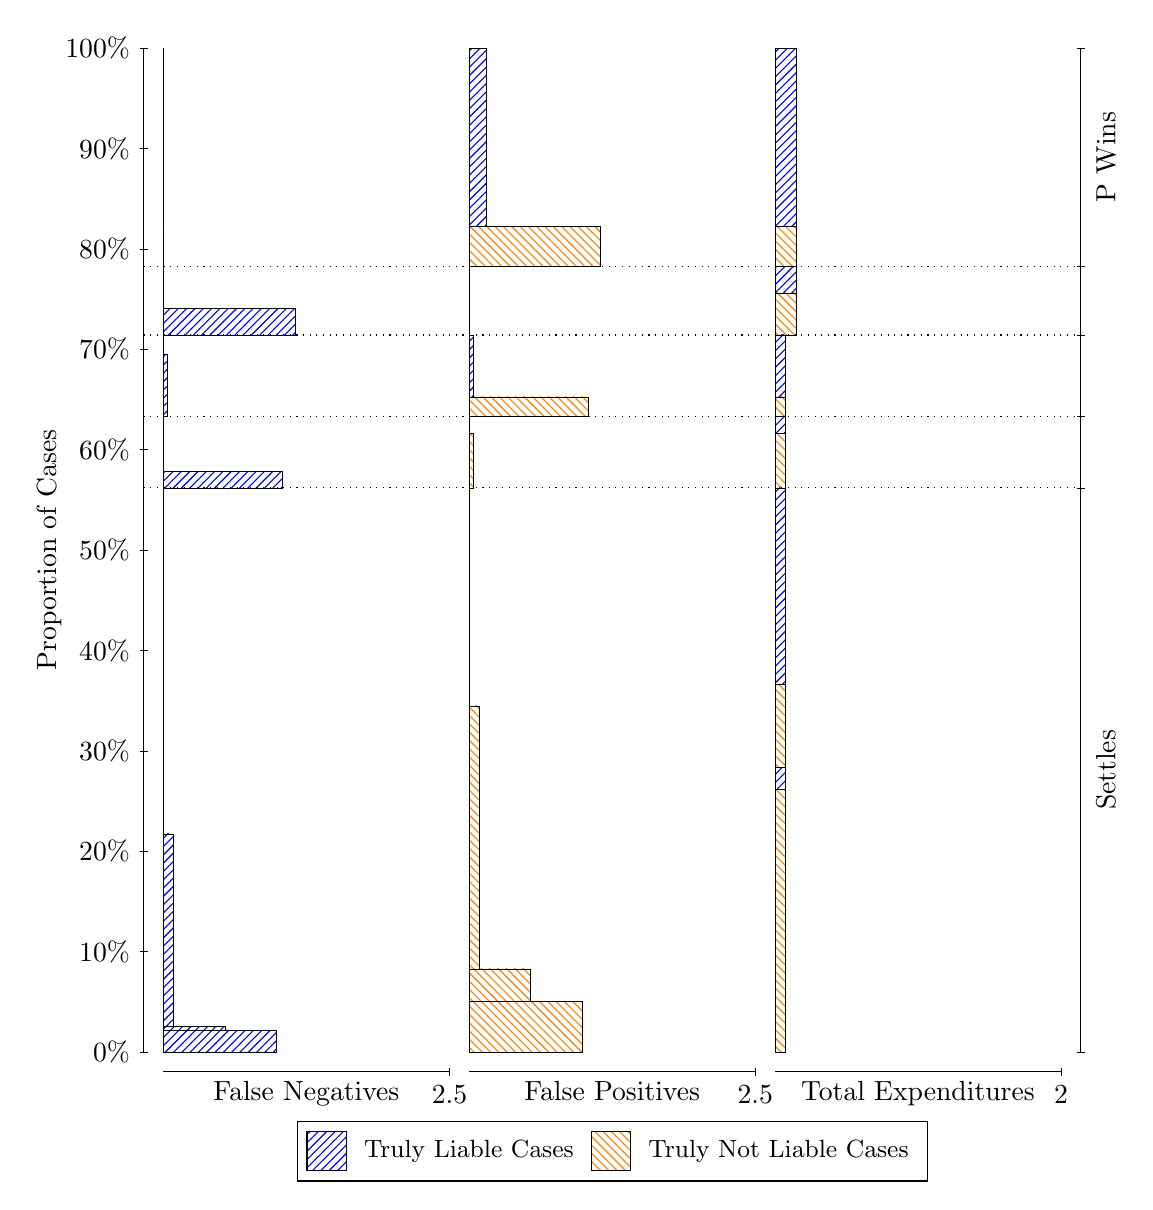
\begin{tikzpicture}
\draw[black, very thin] (1.5,1.75) -- (1.5,14.5);
\node[rotate=90, text=black, anchor=center] at (0.3, 8.125) {Proportion of Cases};
\draw[black, very thin] (1.45,1.75) -- (1.55,1.75);
\node[text=black, anchor=east] at (1.45, 1.75) {0\%};
\draw[black, very thin] (1.45,3.025) -- (1.55,3.025);
\node[text=black, anchor=east] at (1.45, 3.025) {10\%};
\draw[black, very thin] (1.45,4.3) -- (1.55,4.3);
\node[text=black, anchor=east] at (1.45, 4.3) {20\%};
\draw[black, very thin] (1.45,5.575) -- (1.55,5.575);
\node[text=black, anchor=east] at (1.45, 5.575) {30\%};
\draw[black, very thin] (1.45,6.85) -- (1.55,6.85);
\node[text=black, anchor=east] at (1.45, 6.85) {40\%};
\draw[black, very thin] (1.45,8.125) -- (1.55,8.125);
\node[text=black, anchor=east] at (1.45, 8.125) {50\%};
\draw[black, very thin] (1.45,9.4) -- (1.55,9.4);
\node[text=black, anchor=east] at (1.45, 9.4) {60\%};
\draw[black, very thin] (1.45,10.675) -- (1.55,10.675);
\node[text=black, anchor=east] at (1.45, 10.675) {70\%};
\draw[black, very thin] (1.45,11.95) -- (1.55,11.95);
\node[text=black, anchor=east] at (1.45, 11.95) {80\%};
\draw[black, very thin] (1.45,13.225) -- (1.55,13.225);
\node[text=black, anchor=east] at (1.45, 13.225) {90\%};
\draw[black, very thin] (1.45,14.5) -- (1.55,14.5);
\node[text=black, anchor=east] at (1.45, 14.5) {100\%};

\draw[black, very thin] (13.4,1.75) -- (13.4,14.5);
\draw[black, very thin] (13.35,1.75) -- (13.45,1.75);
\node[anchor=west] at (13.35, 1.75) {};
\draw[black, very thin] (13.35,8.9138) -- (13.45,8.9138);
\node[anchor=west] at (13.35, 8.9138) {};
\draw[black, very thin] (13.35,9.8242) -- (13.45,9.8242);
\node[anchor=west] at (13.35, 9.8242) {};
\draw[black, very thin] (13.35,10.856) -- (13.45,10.856);
\node[anchor=west] at (13.35, 10.856) {};
\draw[black, very thin] (13.35,11.729) -- (13.45,11.729);
\node[anchor=west] at (13.35, 11.729) {};
\draw[black, very thin] (13.35,14.5) -- (13.45,14.5);
\node[anchor=west] at (13.35, 14.5) {};

\draw[black, very thin, pattern color=blue, pattern=north east lines] (1.75,1.75) rectangle (3.1852,2.0275);
\draw[black, very thin, pattern color=blue, pattern=north east lines] (1.75,2.0275) rectangle (2.5312,2.0755);
\draw[black, very thin, pattern color=blue, pattern=north east lines] (1.75,2.0755) rectangle (1.8772,4.5196);
\draw[black, very thin, pattern color=orange, pattern=north west lines] (1.75,4.5196) rectangle (1.75,8.9138);
\draw[black, very thin, pattern color=blue, pattern=north east lines] (1.75,8.9138) rectangle (3.2578,9.1272);
\draw[black, very thin, pattern color=orange, pattern=north west lines] (1.75,9.1272) rectangle (1.75,9.8242);
\draw[black, very thin, pattern color=blue, pattern=north east lines] (1.75,9.8242) rectangle (1.8045,10.611);
\draw[black, very thin, pattern color=orange, pattern=north west lines] (1.75,10.611) rectangle (1.75,10.856);
\draw[black, very thin, pattern color=blue, pattern=north east lines] (1.75,10.856) rectangle (3.4213,11.196);
\draw[black, very thin, pattern color=orange, pattern=north west lines] (1.75,11.196) rectangle (1.75,11.729);
\draw[black, very thin, pattern color=orange, pattern=north west lines] (1.75,11.729) rectangle (1.75,12.234);
\draw[black, very thin, pattern color=blue, pattern=north east lines] (1.75,12.234) rectangle (1.75,14.5);
\draw[black, very thin, pattern color=orange, pattern=north west lines] (5.6333,1.75) rectangle (7.0685,2.3876);
\draw[black, very thin, pattern color=orange, pattern=north west lines] (5.6333,2.3876) rectangle (6.4145,2.8057);
\draw[black, very thin, pattern color=orange, pattern=north west lines] (5.6333,2.8057) rectangle (5.7605,6.1442);
\draw[black, very thin, pattern color=blue, pattern=north east lines] (5.6333,6.1442) rectangle (5.6333,8.9138);
\draw[black, very thin, pattern color=orange, pattern=north west lines] (5.6333,8.9138) rectangle (5.6878,9.6108);
\draw[black, very thin, pattern color=blue, pattern=north east lines] (5.6333,9.6108) rectangle (5.6333,9.8242);
\draw[black, very thin, pattern color=orange, pattern=north west lines] (5.6333,9.8242) rectangle (7.1412,10.07);
\draw[black, very thin, pattern color=blue, pattern=north east lines] (5.6333,10.07) rectangle (5.6878,10.856);
\draw[black, very thin, pattern color=orange, pattern=north west lines] (5.6333,10.856) rectangle (5.6333,11.389);
\draw[black, very thin, pattern color=blue, pattern=north east lines] (5.6333,11.389) rectangle (5.6333,11.729);
\draw[black, very thin, pattern color=orange, pattern=north west lines] (5.6333,11.729) rectangle (7.3047,12.234);
\draw[black, very thin, pattern color=blue, pattern=north east lines] (5.6333,12.234) rectangle (5.8513,14.5);
\draw[black, very thin, pattern color=orange, pattern=north west lines] (9.5167,1.75) rectangle (9.6529,5.0884);
\draw[black, very thin, pattern color=blue, pattern=north east lines] (9.5167,5.0884) rectangle (9.6529,5.366);
\draw[black, very thin, pattern color=orange, pattern=north west lines] (9.5167,5.366) rectangle (9.6529,6.4217);
\draw[black, very thin, pattern color=blue, pattern=north east lines] (9.5167,6.4217) rectangle (9.6529,8.9138);
\draw[black, very thin, pattern color=orange, pattern=north west lines] (9.5167,8.9138) rectangle (9.6529,9.6108);
\draw[black, very thin, pattern color=blue, pattern=north east lines] (9.5167,9.6108) rectangle (9.6529,9.8242);
\draw[black, very thin, pattern color=orange, pattern=north west lines] (9.5167,9.8242) rectangle (9.6529,10.07);
\draw[black, very thin, pattern color=blue, pattern=north east lines] (9.5167,10.07) rectangle (9.6529,10.856);
\draw[black, very thin, pattern color=orange, pattern=north west lines] (9.5167,10.856) rectangle (9.7892,11.389);
\draw[black, very thin, pattern color=blue, pattern=north east lines] (9.5167,11.389) rectangle (9.7892,11.729);
\draw[black, very thin, pattern color=orange, pattern=north west lines] (9.5167,11.729) rectangle (9.7892,12.234);
\draw[black, very thin, pattern color=blue, pattern=north east lines] (9.5167,12.234) rectangle (9.7892,14.5);
\draw[black, dotted] (1.5,8.9138) -- (13.4,8.9138);
\draw[black, dotted] (1.5,9.8242) -- (13.4,9.8242);
\draw[black, dotted] (1.5,10.856) -- (13.4,10.856);
\draw[black, dotted] (1.5,11.729) -- (13.4,11.729);
\draw[black, very thin] (1.75,1.5) -- (5.3833,1.5);
\node[text=black, anchor=north] at (3.5667, 1.5) {False Negatives};
\draw[black, very thin] (5.3833,1.45) -- (5.3833,1.55);
\node[text=black, anchor=north] at (5.3833, 1.45) {2.5};

\draw[black, very thin] (5.6333,1.5) -- (9.2667,1.5);
\node[text=black, anchor=north] at (7.45, 1.5) {False Positives};
\draw[black, very thin] (9.2667,1.45) -- (9.2667,1.55);
\node[text=black, anchor=north] at (9.2667, 1.45) {2.5};

\draw[black, very thin] (9.5167,1.5) -- (13.15,1.5);
\node[text=black, anchor=north] at (11.333, 1.5) {Total Expenditures};
\draw[black, very thin] (13.15,1.45) -- (13.15,1.55);
\node[text=black, anchor=north] at (13.15, 1.45) {2};

\node[text=black, centered, rotate=90] at (13.72, 5.3319) {Settles};



\node[text=black, centered, rotate=90] at (13.72, 13.114) {P Wins};

\draw (7.449999999999999,1.5) node[draw=none] (baseCoordinate) {};
\begin{scope}[align=center]
        \matrix[scale=0.5, draw=black, below=0.5cm of baseCoordinate, nodes={draw}, column sep=0.1cm]{
            \node[rectangle, draw, minimum width=0.5cm, minimum height=0.5cm, pattern color=blue, pattern=north east lines] {}; &
            \node[draw=none, font=\small, text=black] (B) {Truly Liable Cases}; &
            \node[rectangle, draw, minimum width=0.5cm, minimum height=0.5cm, pattern color=orange, pattern=north west lines] {}; &
            \node[draw=none, font=\small, text=black] (B) {Truly Not Liable Cases}; \\
            };
\end{scope}

\end{tikzpicture}
\end{document}